\section{Processi primari}
In questa sezione vengono descritti i processi di fornitura e sviluppo messi in atto dal gruppo di lavoro \GRUPPO. Il processo di acquisizione spetta al Committente e al Proponente del capitolato scelto, mentre il processo di manutenzione non può essere eseguito per vincoli dati dal tempo disponibile. Ad ogni modo, il prodotto \textit{software} e la documentazione fornita devono garantire la possibilità futura di essere sottoposti alle attività previste dal processo di manutenzione.
\subsection{Fornitura}
\subsubsection{Attività}
\paragraph{Accettazione}
\subparagraph{Discussione e scelta del capitolato}
Il \textit{Responsabile di Progetto} ha il compito di organizzare gli incontri per permettere ai componenti del gruppo di discutere sui capitolati disponibili.
Le valutazioni che hanno portato a prendere una decisione finale sono documentate nello \textit{Studio di Fattibilità v1.0.0}.
\subparagraph{Studio di fattibilità}
Per realizzare il documento devono essere presi in considerazione i seguenti punti, adattati ai capitolati disponibili:
\begin{itemize}
\item{Valutazione generale del capitolato;}
\item{Valutazione dei fattori di rischio.}
\end{itemize}

Per il capitolato scelto devono essere analizzati anche i seguenti punti:
\begin{itemize}
	\item{Studio del dominio applicativo;}
	\item{Studio del dominio tecnologico;}
	\item{Analisi di mercato;}
	\item{Analisi delle potenziali criticità.}
\end{itemize}

\paragraph{Preparazione della risposta}
\subparagraph{Definizione e preparazione della proposta}
I membri del gruppo \GRUPPO\ devono redigere i seguenti documenti:
\begin{itemize}
	\item{Norme di Progetto;}
	\item{Studio di Fattibilità;}
	\item{Analisi dei Requisiti;}
	\item{Piano di Progetto;}
	\item{Piano di Qualifica.}
\end{itemize}
In allegato viene consegnata anche la \textit{Lettera di Presentazione}. Si veda la sezione \hyperref[sec:versionamento]{3.1.4.2 Versionamento} per maggiori dettagli sul numero di versione indicato nei documenti.

\paragraph{Pianificazione}
\subparagraph{Scelta del modello di ciclo di vita}
Il \textit{Responsabile di Progetto} ha il compito di scegliere il modello di ciclo di vita\G\ più consono allo sviluppo del prodotto richiesto, a meno che non vengano fornite indicazioni specifiche da parte del Proponente.
\subparagraph{Sviluppo e documentazione del Piano di Progetto}
Il \textit{Responsabile di Progetto} ha il compito di delineare i lavori che i membri del gruppo sono incaricati a eseguire. Inoltre deve calcolare costi e tempistiche per le attività da svolgere. Tali pianificazioni sono riportate nel documento \textit{Piano di Progetto v1.0.0}.

\subsection{Sviluppo}
Il processo di sviluppo contiene tutte le attività coinvolte nella realizzazione del prodotto \textit{software} e svolte dal gruppo \GRUPPO.

\subsubsection{Attività}
\paragraph{Analisi dei requisiti}
Dopo aver redatto lo \textit{Studio di Fattibilità}, gli \textit{Analisti} hanno l'incarico di produrre il documento \textit{Analisi dei Requisiti v1.0.0}. L'obiettivo è produrre dei requisiti a partire dalle informazioni acquisite dal gruppo.
Le risorse elaborate a questo scopo provengono da uno studio del capitolato d'appalto e come risultato di eventuali incontri con Proponente e Committente.

\subsubsection{Norme}
\paragraph{Classificazione dei requisiti}
I requisiti prodotti devono essere classificati a seconda del tipo e dell'importanza, rispettando la seguente notazione:
\begin{center}
	R[Importanza][Tipo][Codice]
\end{center}

\begin{itemize}
	\item\textbf{Importanza}: i valori che può assumere sono:
	
	\begin{itemize}
		\item[-] 0: requisito obbligatorio;
		\item[-] 1: requisito desiderabile;
		\item[-] 2: requisito opzionale.
	\end{itemize}
	
	\item\textbf{Tipo}: i valori che può assumere sono:
		\begin{itemize}
			\item[-] F: requisito funzionale;
			\item[-] P: requisito prestazionale;
			\item[-] Q: requisito di qualità;
			\item[-] V: requisito di vincolo.
		\end{itemize}
	
	\item\textbf{Codice}: è il codice gerarchico e univoco del vincolo espresso nella forma X.Y.Z dove X, Y e Z sono dei valori numerici.
\end{itemize}
Inoltre, ogni requisito deve contenere le seguenti informazioni:
	
\begin{itemize}
	\item\textbf{Descrizione}: descrizione del requisito con la minore ambiguità possibile;
	\item\textbf{Fonte}: la scelta può ricadere tra:
	\begin{itemize}
		\item[-] \textbf{Capitolato}: requisito ottenuto dalle specifiche del capitolato;
		\item[-] \textbf{Interno}: requisito elaborato dagli \textit{Analisti} nel corso di un'analisi più approfondita del problema;
		\item[-] \textbf{Caso d'uso}: requisito ottenuto da uno o più casi d'uso. Deve essere quindi specificato il codice del caso d'uso a cui ci si riferisce;
		\item[-] \textbf{Verbale}: requisito ottenuto da un incontro con il Proponente o da riunioni interne tra i membri del gruppo di lavoro \GRUPPO.
	\end{itemize}
\end{itemize}

\paragraph{Classificazione dei casi d'uso}
I casi d'uso devono essere suddivisi in ordine gerarchico secondo il seguente schema:
\begin{center}
	UC[Codice]
\end{center}

	\begin{itemize}
		\item \textbf{Codice}: è il codice gerarchico e univoco che serve a identificare ogni caso d'uso.
	\end{itemize}
Per ogni caso d'uso devono essere presenti anche le seguenti informazioni:
	\begin{itemize}
		\item \textbf{Titolo}: è necessario fornire un titolo riassuntivo dell'operazione che il caso d'uso intende modellare;
		\item \textbf{Descrizione}: è necessario fornire una breve descrizione con la minore ambiguità possibile;
		\item \textbf{Attori}: elenco degli attori coinvolti nel caso d'uso;
		\item \textbf{Scenari principali}: descrizione dei possibili scenari principali;
		\item \textbf{Scenari alternativi}: descrizione dei possibili scenari secondari;
		\item \textbf{Pre-condizioni}: una pre-condizione è una condizione sempre vera all'inizio del caso d'uso;
		\item \textbf{Flusso degli eventi}: ordine di esecuzione dei casi d'uso figli;
		\item \textbf{Inclusioni}: spiegazione di tutte le inclusioni se presenti;
		\item \textbf{Estensioni}: spiegazione di tutte le estensioni se presenti;
		\item \textbf{Generalizzazioni}: spiegazione di tutte le generalizzazioni se presenti;
		\item \textbf{Post-condizioni}: una post-condizione è una condizione sempre vera alla fine dell'esecuzione del caso d'uso.
	\end{itemize}
Alcune fra le precedenti informazioni potrebbero essere assenti nel caso non fossero utilizzate.

\paragraph{Codifica dei file}
Tutti i \textit{file} creati dal gruppo che contengono codice e che fanno parte della documentazione devono essere codificati tramite UTF-8\G\ senza BOM\G. Eventuali cambiamenti di codifica devono essere approvati dal \textit{Responsabile di Progetto}.
\paragraph{Nomi e norme di codifica}
Questa sezione verrà redatta nel dettaglio durante le fasi di consegna successive alla Revisione dei Requisiti. Vengono introdotte alcune norme da rispettare durante lo sviluppo del codice, indipendentemente dal linguaggio di programmazione che verrà adottato. Le norme introdotte sono le seguenti:

\begin{itemize}
	\item In ogni \textit{file} deve essere presente un'intestazione contenente le seguenti informazioni: 
	\begin{itemize}
		\item[-] Percorso e nome del \textit{file};
		\item[-] Nome e cognome dell'autore;
		\item[-] Data di creazione;
		\item[-] Indirizzo email dell’autore;
		\item[-] Per ogni modifica effettuata devono essere specificati: la versione successiva generata dall'avanzamento, l'autore, la data e una breve descrizione.	
	\end{itemize}
	\item I nomi delle variabili devono essere chiari, descrittivi e in inglese;
	\item I commenti vanno scritti in italiano.
\end{itemize}

\paragraph{Ricorsione}
Quando possibile, la ricorsione va evitata. Per ogni funzione ricorsiva è d'obbligo fornire una prova di terminazione. Inoltre risulta necessario valutare il costo in termini di occupazione della memoria. Nel caso in cui l'utilizzo di memoria risulti eccessivo, la ricorsione deve essere rimossa.
\subsubsection{Strumenti}

\paragraph{Inserimento dei requisiti}
Per tenere traccia dei requisiti è stato sviluppato un semplice servizio \textit{web} accessibile ai soli membri del gruppo presso l'indirizzo
\begin{center}
	\url{www.starklabs.altervista.org} \\
\end{center}
Lo strumento realizzato si basa su un \textit{database}\G\ in MySQL\G\ nel quale sono memorizzate tutte le informazioni riguardanti casi d'uso e requisiti. Di seguito vengono descritte le tabelle più significative del \textit{database}:
\begin{itemize}
\item \textbf{Tabella dei casi d'uso}: in essa sono presenti:
	\begin{itemize}
		 \item [-] Nome del caso d'uso;
		 \item [-] Descrizione del caso d'uso;
		 \item [-] Attori relativi al caso d'uso; 
		 \item [-] Ambito del caso d'uso, espresso in forma numerica, con 1 che rappresenta l'applicazione per gli sceneggiati, 2 l'applicazione di configurazione e 3 il modulo di sistema; 
		 \item [-] Codice univoco che tiene traccia del caso d'uso.
	\end{itemize}
\item \textbf{Tabella dei requisiti}: in essa sono presenti: 
	\begin{itemize}
		\item [-] ID per tenere traccia dell'ordine di inserimento dei requisiti;
		\item [-] Descrizione del requisito;
		\item [-] Importanza del requisito;
		\item [-] Tipologia del requisito;
		\item [-] Codice del requisito, generato tramite PHP\G\ in modo dinamico dopo l'inserimento effettuato dall'interfaccia del servizio. Il codice può mutare nel tempo e rimane definitivo una volta che tutti i requisiti sono stati inseriti.
	\end{itemize}
\end{itemize}
Nel suddetto sito è presente una pagina Requisiti dove è disponibile lo strumento creato per inserire casi d'uso e requisiti. L'interfaccia di inserimento dei casi d'uso è strutturata nel seguente modo ed è inoltre mostrata in \hyperref[sec:Figura1]{Figura 1}:
\begin{itemize}
	\item \textbf{Attori}: area di testo per l'inserimento degli attori;
	\item \textbf{Nome UC}: area di testo per l'inserimento del nome del caso d'uso;
	\item \textbf{Codice UC}: area di testo per l'inserimento del codice del caso d'uso;
	\item \textbf{Visione di dettaglio dell'UC}: menu a tendina per la selezione del caso d'uso più generico da cui deriva un caso d'uso più specifico;
	\item \textbf{Ambito}: menu a tendina per la selezione dell'ambito del caso d'uso;
	\item \textbf{Descrizione}: area di testo per l'inserimento della descrizione del caso d'uso;
	\item \textbf{Inclusione dell'UC}: menu a tendina per la selezione del caso d'uso verso cui si fa inclusione;
	\item \textbf{Estende l'UC}: menu a tendina per la selezione del caso d'uso verso cui si fa estensione;
	\item \textbf{Commento estensione}: area di testo per l'inserimento di un commento relativo a eventuali estensioni;
	\item \textbf{Generalizza l'UC}: menu a tendina per la selezione del caso d'uso verso cui si fa generalizzazione.
\end{itemize}
L'interfaccia di inserimento dei requisiti è strutturata nel seguente modo ed è invece mostrata in \hyperref[sec:Figura2]{Figura 2}:
\begin{itemize}
	\item \textbf{ID}: area di testo per l'inserimento dell'ID, con suggerimento che suggerisce l'ID subito successivo all'ultimo requisito inserito;
	\item \textbf{Importanza}: menu a tendina per la selezione dell'importanza;
	\item \textbf{Tipologia}: menu a tendina per la selezione della tipologia;
	\item \textbf{Descrizione}: area di testo per l'inserimento della descrizione
	\item \textbf{UC"x"}: fino a cinque menu a tendina per selezionare le dipendenze da cui deriva il requisito, con x che va da 0 a 4;
	\item \textbf{Dipendenza"x"}: fino a cinque menu a tendina per la selezione di dipendenze di un requisito da un altro requisito, con x che va da 0 a 4;
\end{itemize}
Inoltre, viene fornita una funzione che esporta in automatico i contenuti presenti nel \textit{database} all'interno di un documento \LaTeX, che presenta al lettore, in modo ordinato attraverso una tabella, i requisiti inseriti nel database.

\begin{figure}[htbp]
\centering
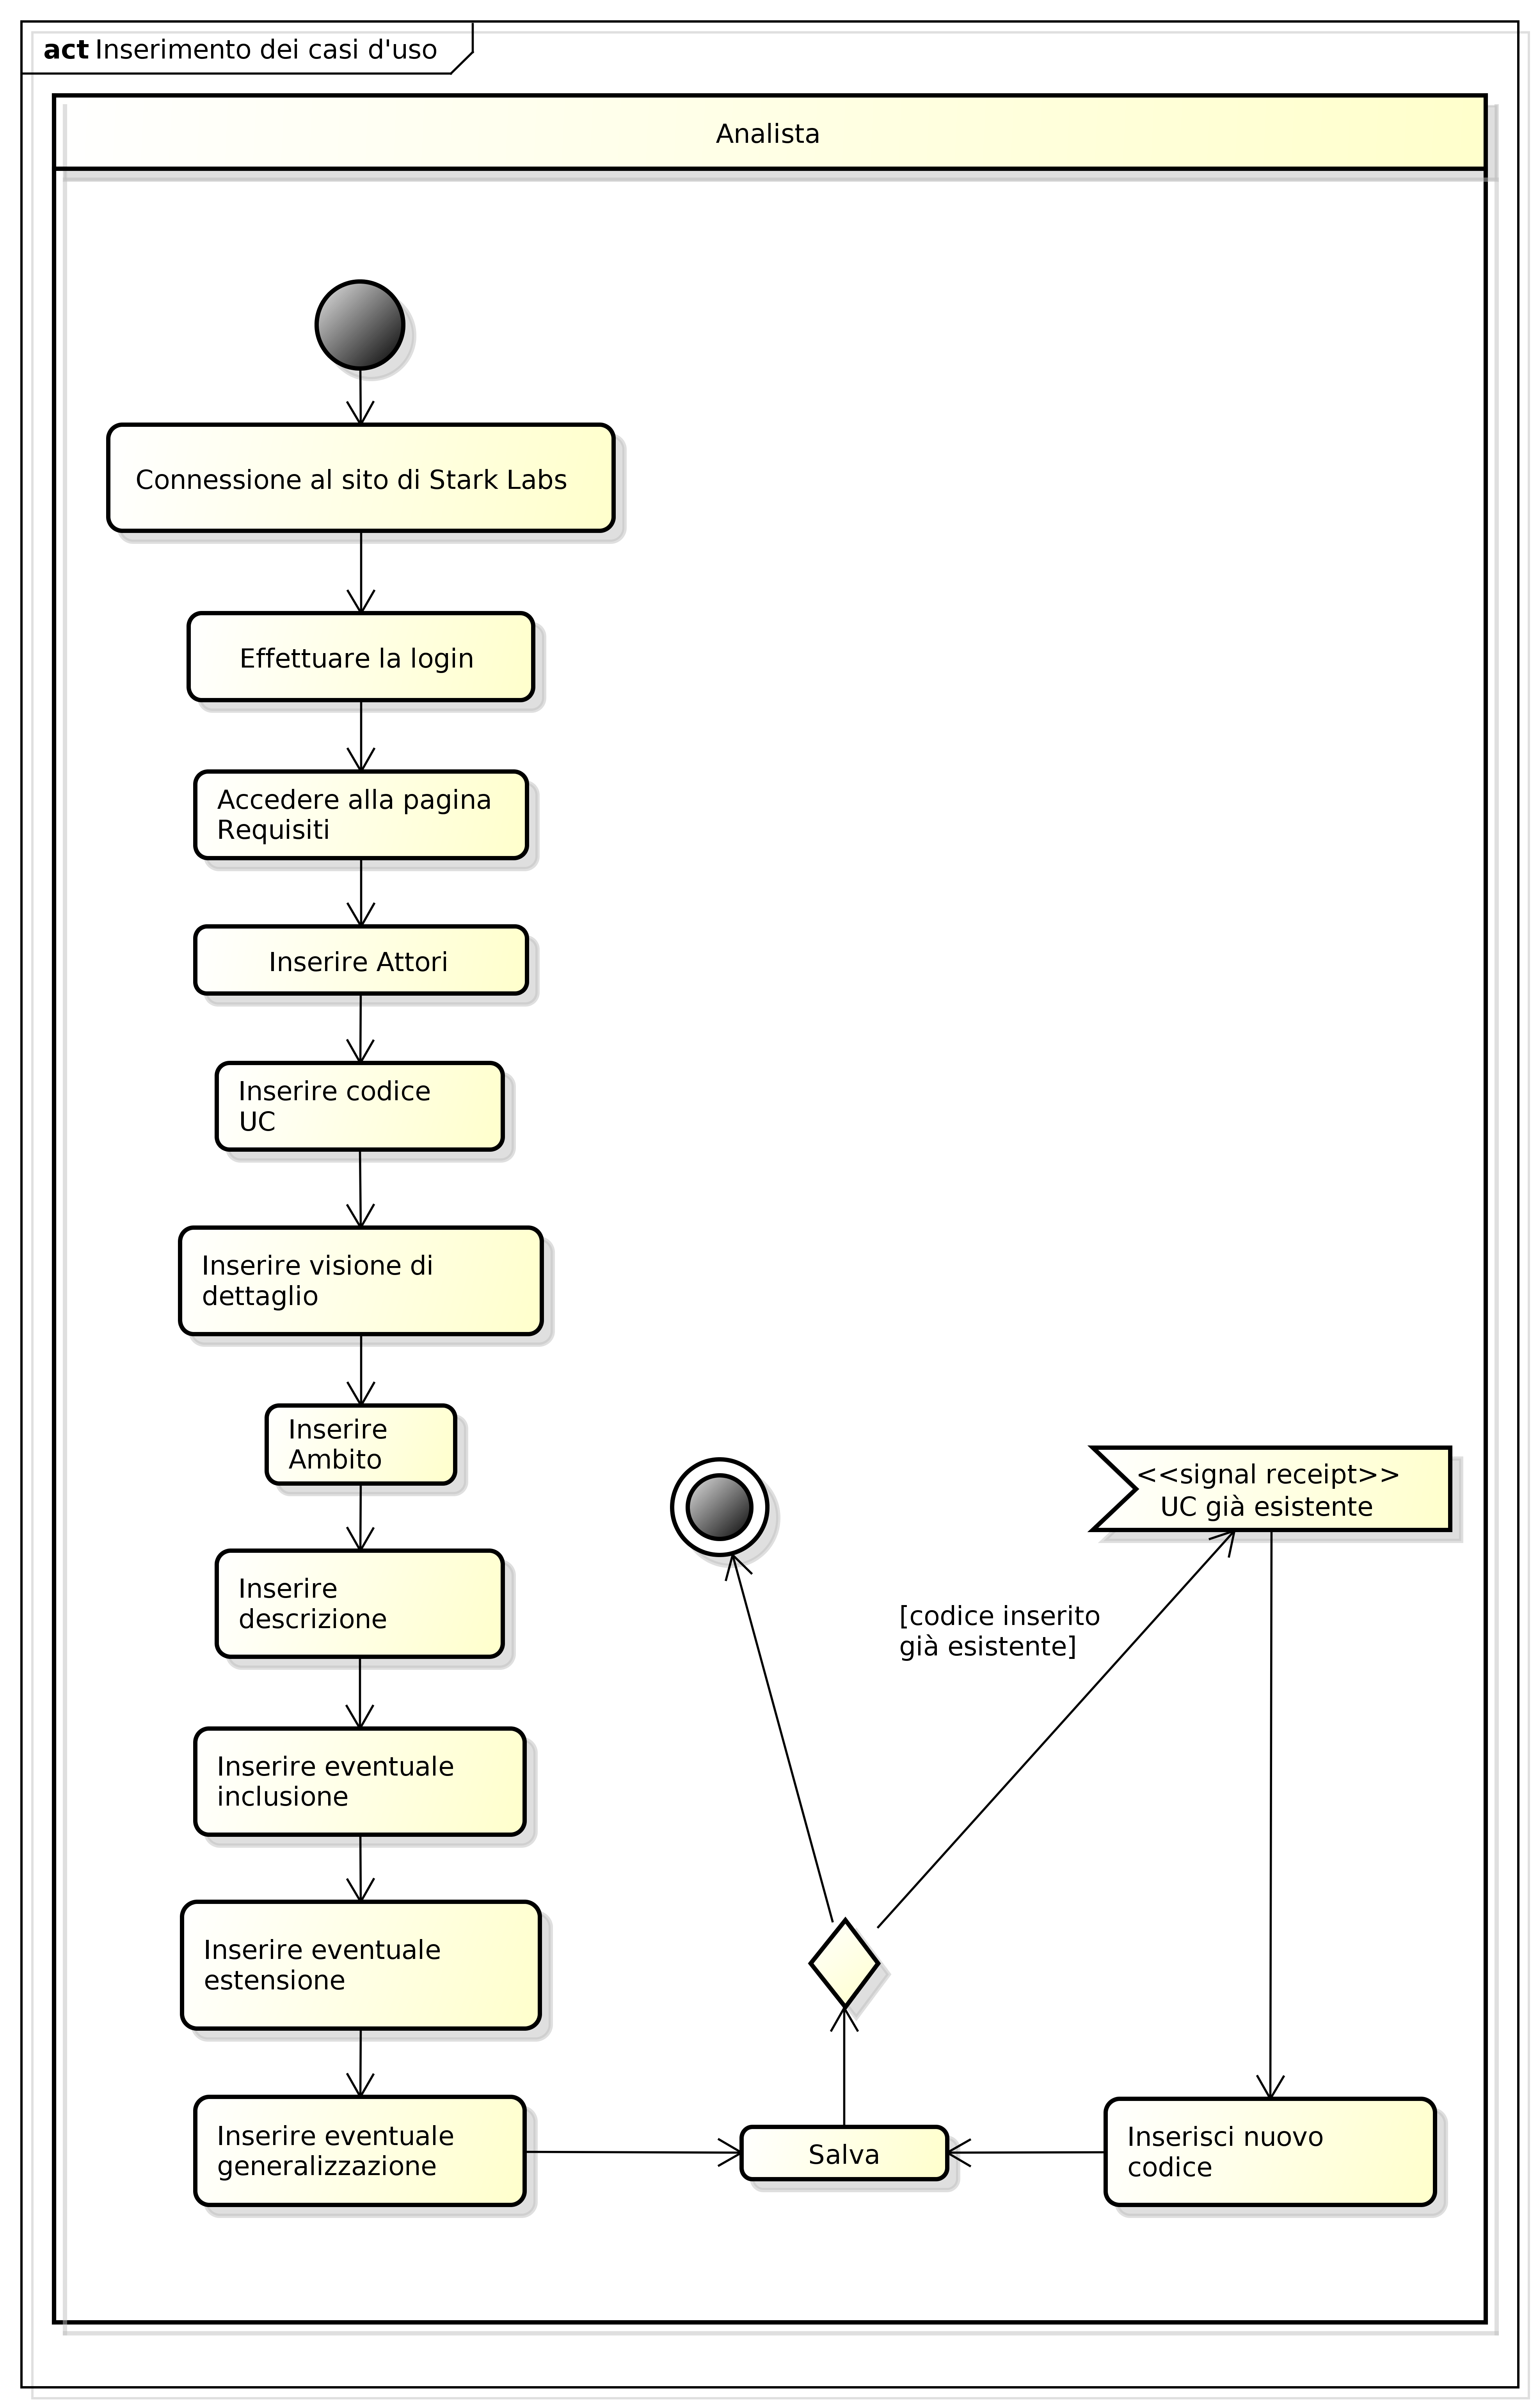
\includegraphics[scale=0.5]{immagini/inserimento_uc.png}
\captionsetup{labelfont=bf}
\caption{Diagramma di attività - Inserimento di un caso d'uso}\label{sec:Figura1}
\end{figure}

\begin{figure}[htbp]
\centering
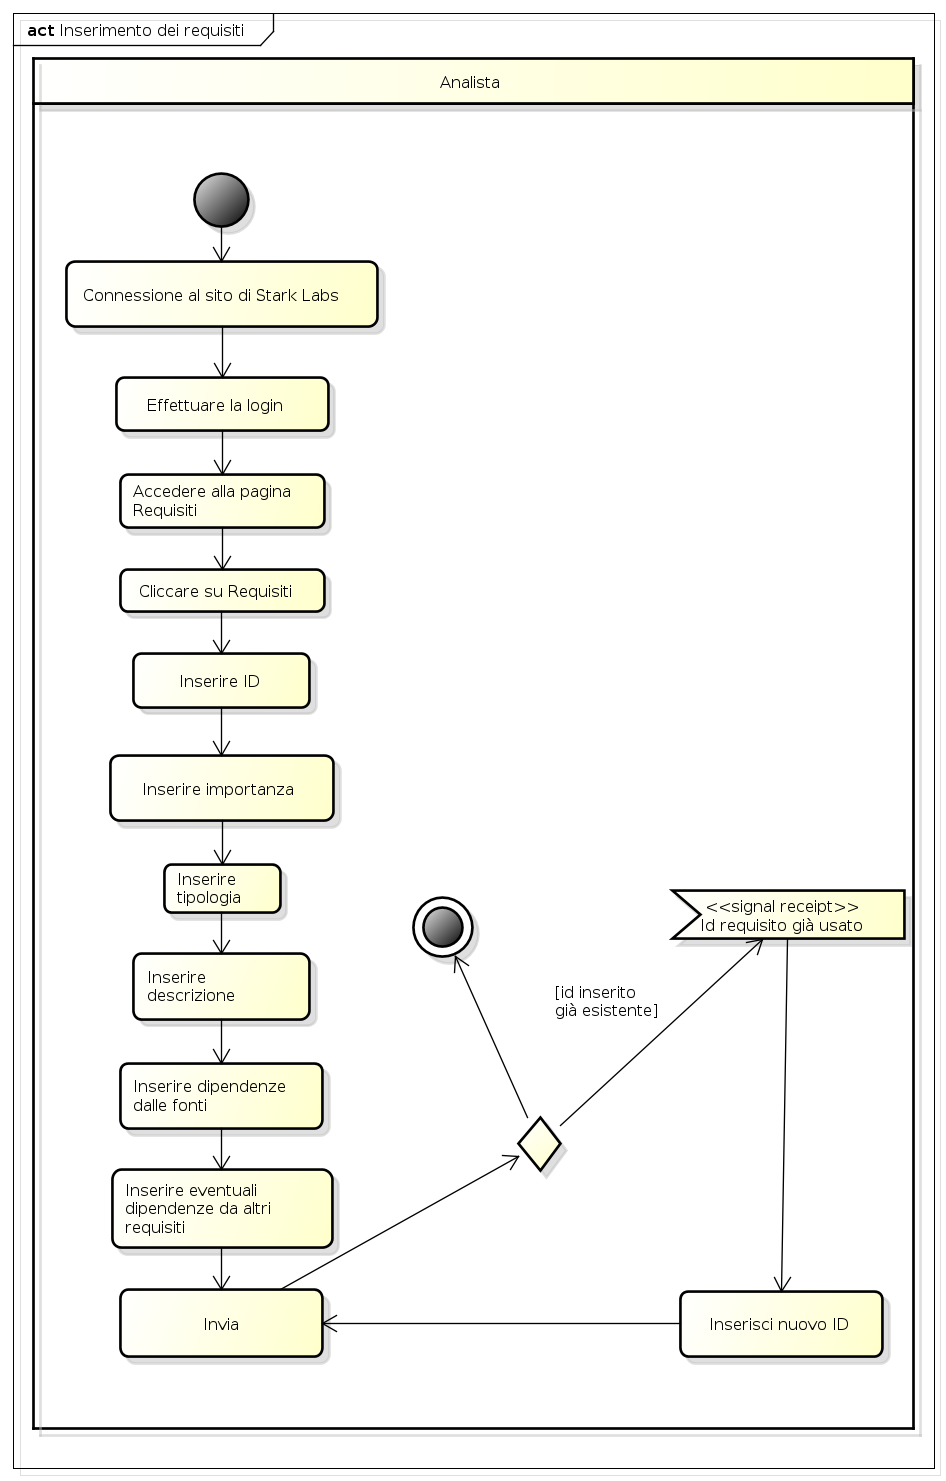
\includegraphics[scale=0.5]{immagini/inserimento_requisiti.png}
\captionsetup{labelfont=bf}
\caption{Diagramma di attività - Inserimento di un requisito}\label{sec:Figura2}
\end{figure}

\newpage
